\documentclass[../paper.tex]{subfiles}
\graphicspath{ {../images/} }

% Document
\begin{document}
    Let's first discuss the data we need to use and the data we used to train our model.
    \subsection{Data}
    Data is the most important part of any machine learning model.
    What data we use to train our model will determine how well our model will perform. 
    There were many things we had to consider when choosing the data. 

    First we looked into custom data, in case we want to make our own dataset. 
    Making our own dataset would have been a good idea, 
    as we could have made the dataset as big and diverse as we wanted.
    The model would be closer to our biases and would fit better to our needs, 
    but the one big disadvantage of making our own dataset, is that it would have taken a lot of time to make a proper dataset. 

    We tried making our own dataset, and made a small working code that could do this automatically, 
    but we quickly realized that it would take too much time considering that one letter per person takes 20\~30 minutes each. 

    We then looked in to different existing datasets, and came across MNIST sign language dataset\cite{d0}. 
    We considered using this dataset, because MNIST is very well known among the machine learning community regarding image classification of letters\cite{o0}.
    The dataset consists of 28$\times$28 images of the American Sign Language alphabet, 
    and has 24 different classes. 
    Some examples listed below:
    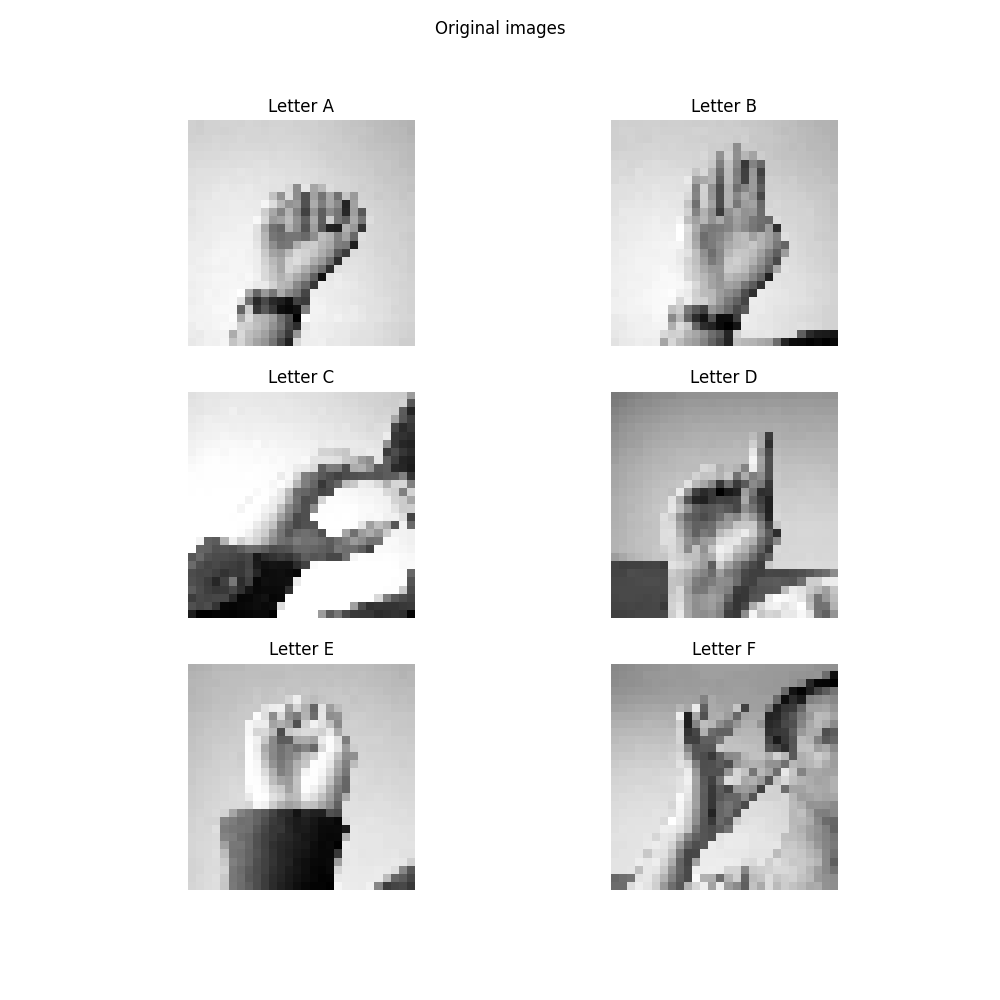
\includegraphics[width=\linewidth]{letters_grid_6} 
    Letter J and Z are not included in the dataset, as they require motion. 

    One problem we later faced is that the dataset was not as big as we wanted it to be,
    we thought of combining this dataset with another dataset, but this would have not been ideal (covered in a later section).

    \subsection{Data preprocessing}
    The dataset was already preprocessed, so we did not have to do any preprocessing on the dataset. 
    We did provide some preprocessing in the code, this is provided in case the dataset is not preprocessed or in case we want to make our own dataset.
    The preprocessing we provide is as follows:
    \begin{itemize} 
        \item We first convert the images to grayscale, as we only need the intensity of the image.
        \item We then resize the images to 28$\times$28, as the images are not all the same size.
        \item We then normalize the images, as the pixel values are between 0 and 255 (in our case remapped between 0 and 1).
    \end{itemize} 
    These are the basic preprocessing steps that are needed, you could add some other preprocessing steps if you want to add blur or noise, etc.
    Accounting that we focus the image first to the hand before we resize.
    We also do some normalization and standardization of the data, as this will help the model to learn better. 
    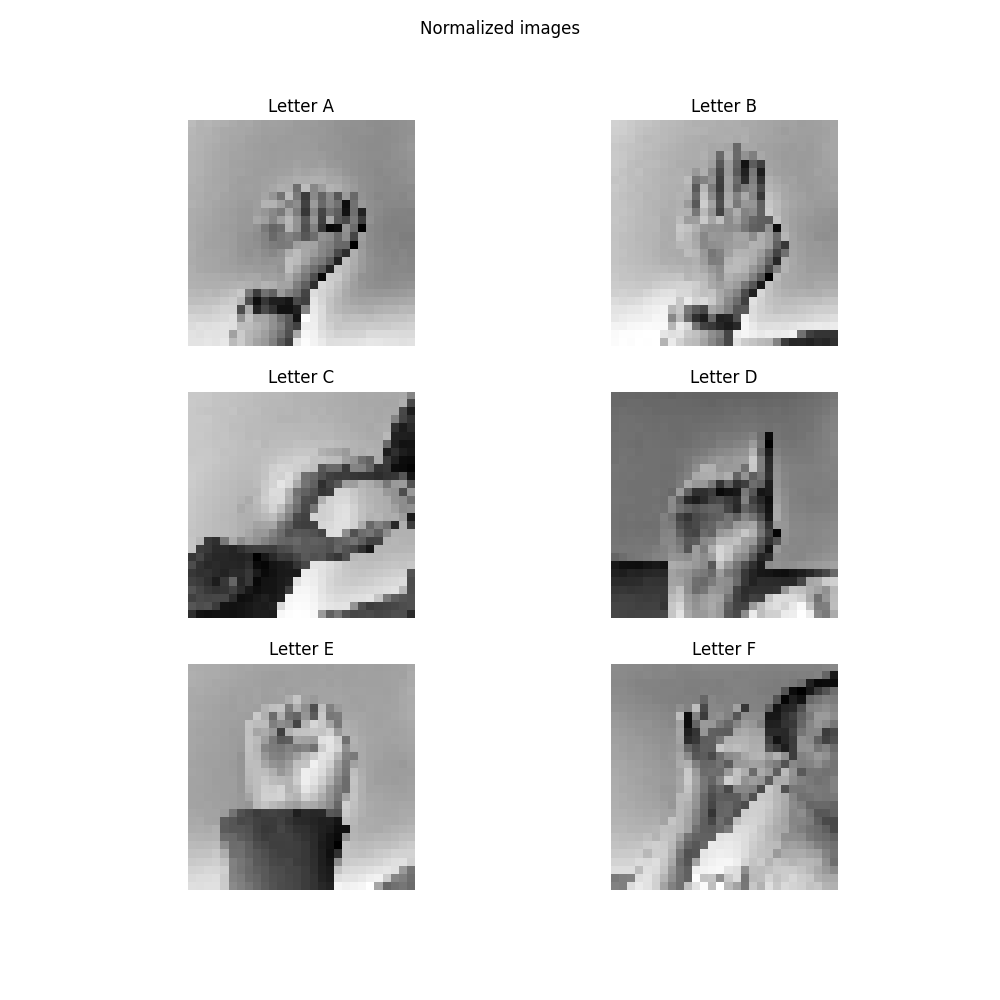
\includegraphics[width=\linewidth]{letters_grid_normalized_6}
    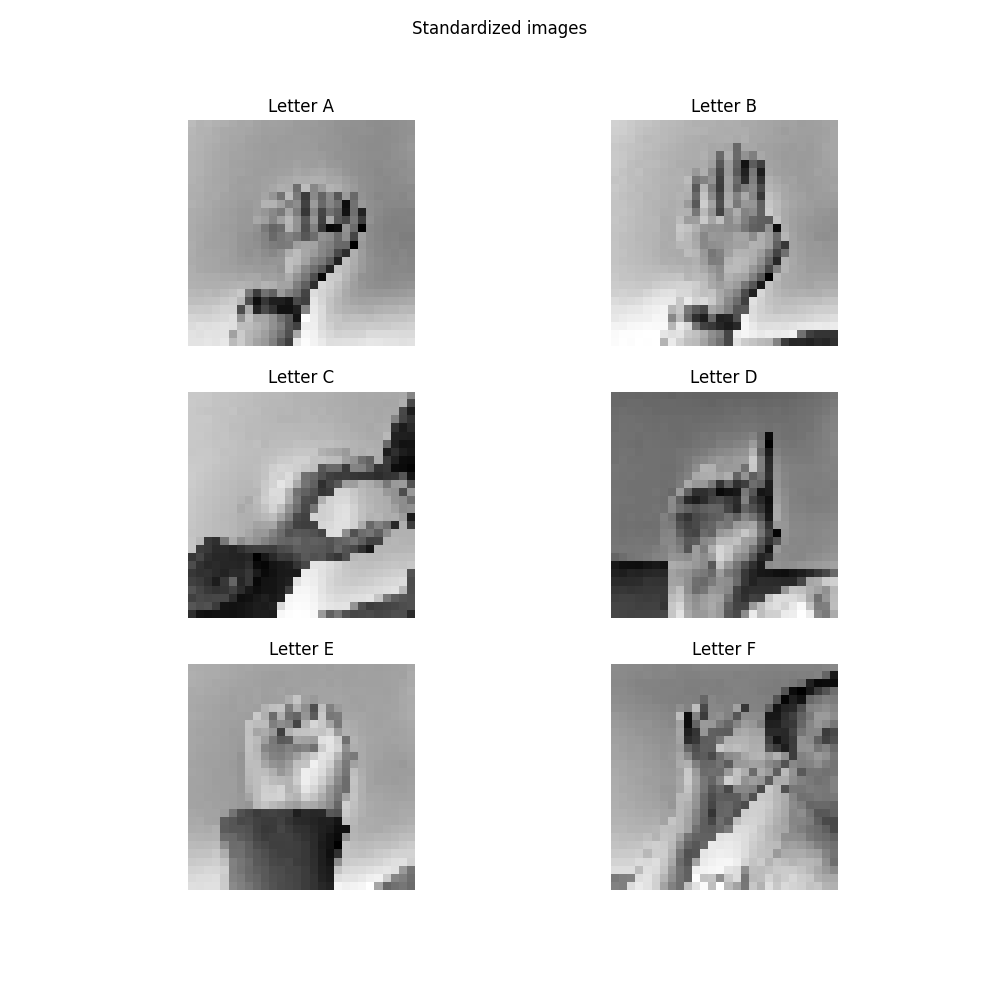
\includegraphics[width=\linewidth]{letters_grid_standardized_6}
    We also make use of a mean image, this is the average of all the images in the dataset.
    We use this image to substract from the images, this will help the model to only focus on the important parts of the image.
    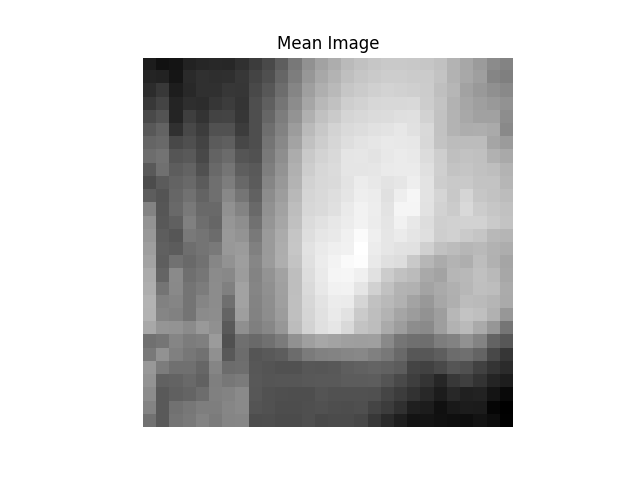
\includegraphics[width=\linewidth]{mean_image_6} 

    This is the preprocessing for the first method, the second method is a bit different, as we need to track the landmarks of the hand first.
    Every hand has 21 landmarks, each landmark signifies a certain point on the hand.
    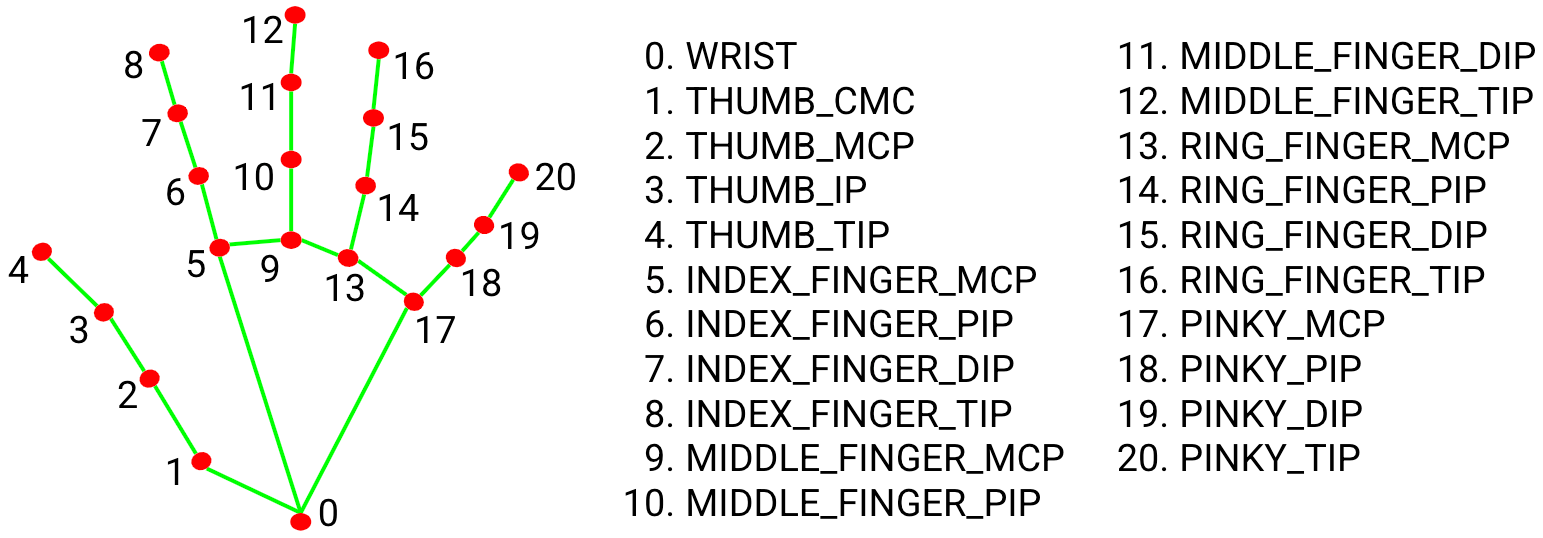
\includegraphics[width=\linewidth]{hand_landmarks}
    Each landmark has a certain x, y and z coordinate, where x is the width, y is the height and z is the depth.

    \subsection{Data formats}
    The dataset itself is in the form of images, and the labels are in the form of integers. 
    After preprocessing the images, we convert the images to an array of pixel values and store this in a csv file. 

    The landmarks are stored in a csv file, where each row is a different image and each column is a different landmark.
    In total there are 21 landmarks on each hand.

    \subsection{Data Augmentation}
    Data augmentation is a technique used to increase the size of the dataset by adding slightly modified copies of the data.
    Note that this could cause problems if not done correctly, the augmentation should still represent realisitic data.

    \subsection{Data distribution}
    We distribute our dataset in a 60\% training set, 30\% validation set and 10\% test set.
    This causes our dataset to be smaller than we would have liked.
    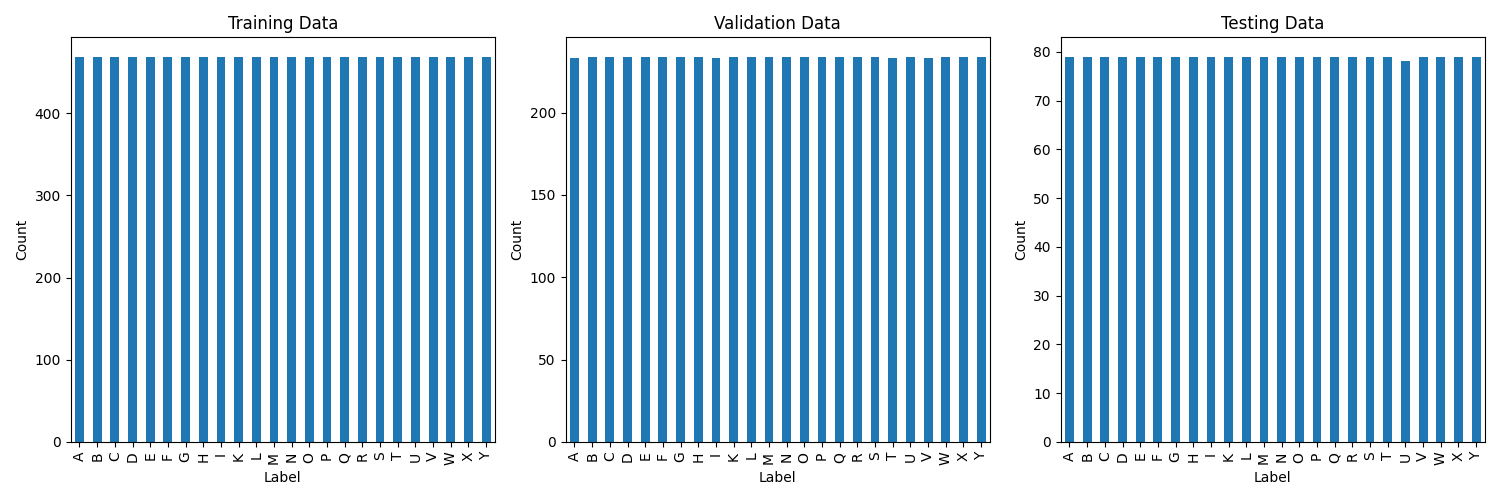
\includegraphics[width=\linewidth]{dataset_distribution}

    \end{document}
